%% tesis.tex — contoh naskah tesis MTI UnLa dengan kelas mti-unla.
%% Kompilasi (disarankan): lualatex tesis → biber tesis → lualatex tesis → lualatex tesis
%% atau cukup: latexmk -lualatex tesis
%% pdfLaTeX dan XeLaTeX juga dapat dipakai (lihat README).
\documentclass{mti-unla}       % tambahkan [satusisi] bila dicetak satu muka (< 115 lembar)

\addbibresource{pustaka.bib}

\judul{Implementasi Deteksi Serangan Jaringan Berbasis Pembelajaran Mesin pada Perangkat Raspberry Pi}
\judulinggris{Implementation of Machine Learning-Based Network Attack Detection on Raspberry Pi Devices}
\penulis{Saleh Wiradikarta}
\npm{L250990001}
\bulantahun{Oktober 2026}
\pembimbingsatu{Prof. Dr. Ir. Dayang Sumbi}
\pembimbingdua{Dr. Ir. Joko Tarub}   % kosongkan bila pembimbing hanya satu
\lambang{logo-unla}

%% Pengecualian pemenggalan khusus naskah ini (tambahkan istilah sendiri):
\babelhyphenation[indonesian]{Rasp-ber-ry}

\begin{document}

%% ================================================================ bagian persiapan
\pagenumbering{roman}
\buathalamanjudul

\begin{abstrak}
Abstrak memuat secara komprehensif permasalahan ilmiah yang diteliti, yang mencakup latar belakang, permasalahan yang dikaji, tujuan, pendekatan dan metode, tahapan penelitian, hasil, serta kesimpulan. Abstrak juga menyebutkan perbandingan hasil dengan penelitian sejenis, menyatakan kebaruan dan orisinalitas penelitian, serta kontribusinya terhadap khazanah ilmu pengetahuan. Abstrak terdiri atas 500--800 kata dan tidak memuat rujukan pustaka, gambar, maupun tabel.

Paragraf berikutnya dipisahkan satu baris kosong dari paragraf sebelumnya.
\katakunci{deteksi intrusi, pembelajaran mesin, Raspberry Pi, keamanan jaringan}
\end{abstrak}

\begin{abstract*}
The abstract is an English translation of the Indonesian abstract. Its title and the whole text are set in italics, and the text is hyphenated with English rules.
\keywords{intrusion detection, machine learning, Raspberry Pi, network security}
\end{abstract*}

\buatpengesahan

\judulbagian{PERNYATAAN KEASLIAN TESIS}
\begin{singlespace}\setlength{\parskip}{12pt}
Dengan ini saya menyatakan bahwa:
\begin{enumerate}[itemsep=6pt]
\item tesis berjudul \enquote{Implementasi Deteksi Serangan Jaringan Berbasis Pembelajaran Mesin pada Perangkat Raspberry Pi} adalah hasil karya saya sendiri dan belum pernah diajukan untuk memperoleh gelar akademik di perguruan tinggi mana pun;
\item tesis ini merupakan gagasan, rumusan, dan hasil penelitian saya sendiri dengan arahan tim pembimbing;
\item dalam tesis ini tidak terdapat karya atau pendapat yang telah ditulis atau dipublikasikan orang lain, kecuali yang secara tertulis dicantumkan sebagai acuan dengan menyebut nama pengarang dan dicantumkan dalam daftar pustaka;
\item penggunaan alat kecerdasan artifisial generatif dalam penyusunan tesis ini telah saya ungkapkan sepenuhnya pada halaman Pernyataan Penggunaan Kecerdasan Artifisial Generatif.
\end{enumerate}
Pernyataan ini saya buat dengan sesungguhnya. Apabila di kemudian hari terdapat penyimpangan dan ketidakbenaran dalam pernyataan ini, saya bersedia menerima sanksi akademik sesuai peraturan yang berlaku di Universitas Langlangbuana.
\end{singlespace}
\begin{tandatangan}
Bandung, \makebox[4cm]{\dotfill}\\
Yang membuat pernyataan,\\[2.5cm]
Saleh Wiradikarta\\
NPM: L250990001
\end{tandatangan}

\judulbagian{PERNYATAAN PENGGUNAAN KECERDASAN ARTIFISIAL GENERATIF}
Isi halaman ini dengan formulir pada Lampiran H pedoman, dalam bentuk formulir atau naratif.

\judulbagian{PEDOMAN PENGGUNAAN TESIS}
Tesis magister yang tidak dipublikasikan terdaftar dan tersedia di Perpustakaan Universitas Langlangbuana, dan terbuka untuk umum dengan ketentuan bahwa hak cipta ada pada penulis dengan mengikuti aturan hak kekayaan intelektual yang berlaku di Universitas Langlangbuana. Referensi kepustakaan diperkenankan dicatat, tetapi pengutipan atau peringkasan hanya dapat dilakukan seizin penulis dan harus disertai kaidah ilmiah untuk menyebutkan sumbernya.

Memperbanyak atau menerbitkan sebagian atau seluruh tesis ini harus seizin Direktur Pascasarjana, Universitas Langlangbuana.

\judulbagian{KATA PENGANTAR}
Penulis sangat berterima kasih kepada Prof. Dr. Ir. Dayang Sumbi dan Dr. Ir. Joko Tarub sebagai pembimbing atas segala saran, bimbingan, dan nasihatnya selama penelitian berlangsung dan selama penulisan tesis ini.

\begin{tandatangan}
Bandung, Oktober 2026\\
Penulis
\end{tandatangan}

\clearpage\tableofcontents
\clearpage\phantomsection\addcontentsline{toc}{chapter}{DAFTAR LAMPIRAN}\listoflampiran
\clearpage\phantomsection\addcontentsline{toc}{chapter}{DAFTAR GAMBAR DAN ILUSTRASI}\listoffigures
\clearpage\phantomsection\addcontentsline{toc}{chapter}{DAFTAR TABEL}\listoftables

\judulbagian{DAFTAR SINGKATAN DAN LAMBANG}
\begin{singlespace}
\begin{longtable}{@{}p{3cm}p{7.1cm}p{3cm}@{}}
\toprule
\textbf{Singkatan/ Lambang} & \textbf{Nama} & \textbf{Pemakaian pertama kali pada halaman}\\ \midrule\endhead
CNN & \asing{Convolutional Neural Network} & \pageref{bab:tinjauan}\\
IDS & \asing{Intrusion Detection System} & 1\\
$F_1$ & rerata harmonik presisi dan perolehan & \pageref{eq:f1}\\ \bottomrule
\end{longtable}
\end{singlespace}

%% ================================================================ tubuh utama
\cleardoublepage
\pagenumbering{arabic}

\chapter{Pendahuluan}\label{bab:pendahuluan}
\section{Latar Belakang}
Perkembangan teknologi informasi dan komunikasi mendorong pemanfaatan perangkat berdaya rendah sebagai bagian dari infrastruktur jaringan. Ketersediaan perangkat seperti \produk{Raspberry Pi} memungkinkan penerapan sistem deteksi intrusi pada tepi jaringan tanpa memerlukan peladen khusus. Namun, keterbatasan sumber daya komputasi menuntut pemilihan algoritma klasifikasi yang tepat agar pengujian, pemantauan, dan pengambilan keputusan dapat dilakukan secara waktu nyata.

Penelitian terdahulu menunjukkan bahwa pendekatan berbasis \asing{machine learning} mampu meningkatkan keakuratan deteksi dibandingkan pendekatan berbasis tanda tangan \parencite{gao2009,kramer2005}. \textcite{kramer2005} menyatakan bahwa pengembangan model yang diimplementasikan pada perangkat terbatas memerlukan penyesuaian arsitektur, sedangkan \textcite{baker1998} menekankan pentingnya pemrosesan awal data. Kutipan langsung disertai halaman, misalnya \parencite[23--25]{baker1998}. Dua karya dari penulis yang sama pada tahun yang sama ditulis \parencite{sumbi2023a,sumbi2023b}.

\section{Rumusan Masalah}
Permasalahan yang dikaji adalah bagaimana merancang, mengimplementasikan, dan mengevaluasi model klasifikasi serangan jaringan yang dapat dijalankan pada perangkat berdaya rendah dengan keakuratan yang memadai.

\section{Tujuan Penelitian}
Uraikan tujuan penelitian.

\section{Metodologi Penelitian}
Tahapan penelitian diperlihatkan pada Gambar~\ref{fig:alir}.
\begin{figure}[htbp]
  \centering
  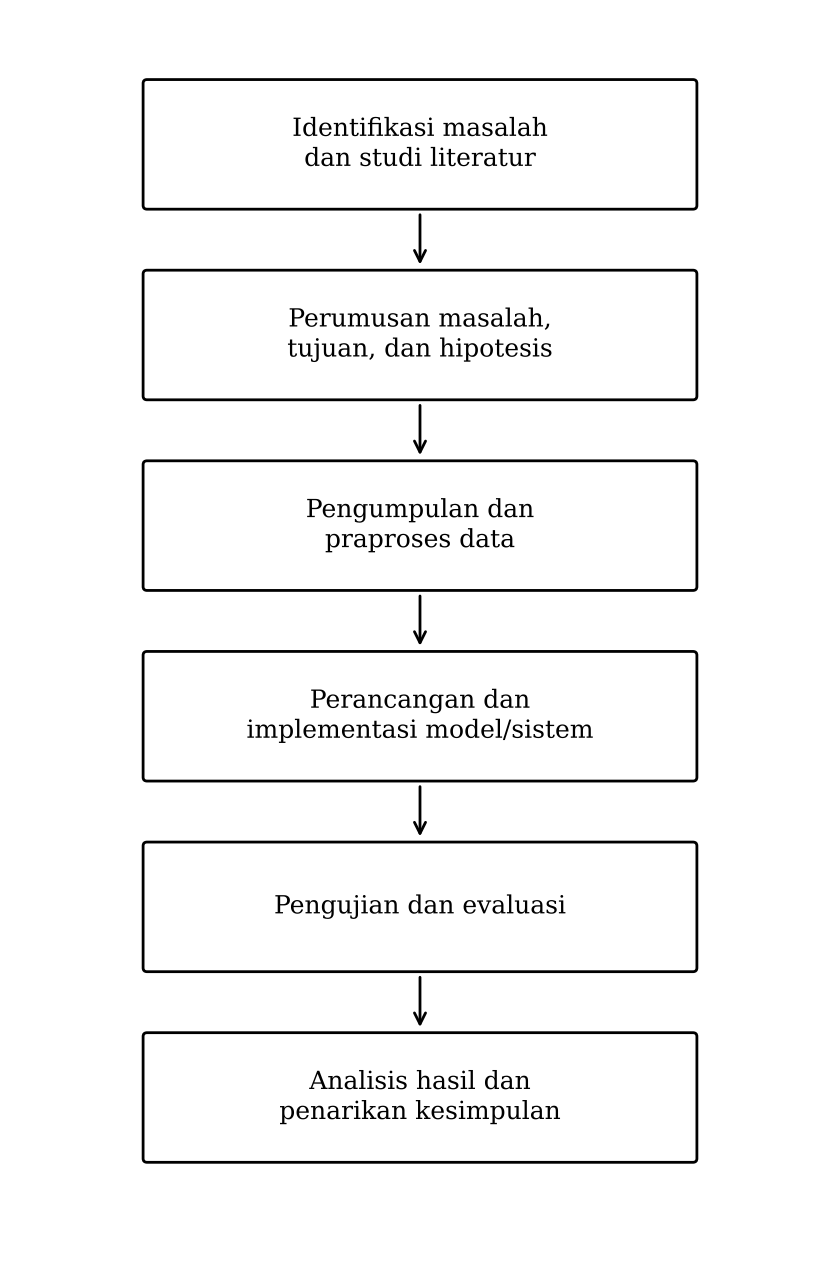
\includegraphics[height=8cm]{alir}
  \caption{Diagram alir penelitian yang dimulai dari identifikasi masalah hingga penarikan kesimpulan (diadaptasi dari \cite{sumbi2023a})}
  \label{fig:alir}
\end{figure}

\chapter{Tinjauan Pustaka}\label{bab:tinjauan}
\section{Landasan Teori}
\subsection{Sistem Deteksi Intrusi}
Sistem deteksi intrusi berbasis anomali membandingkan perilaku lalu lintas jaringan dengan profil normal yang telah dipelajari sebelumnya. Pendekatan ini memungkinkan pengenalan serangan yang belum pernah teridentifikasi, tetapi cenderung menghasilkan alarm palsu yang lebih banyak.

\section{Penelitian Terkait}
Ringkasan penelitian terkait disajikan pada Tabel~\ref{tab:sota}.
\begin{table}[htbp]
  \caption{Perbandingan penelitian terkait}\label{tab:sota}
  \centering
  \begin{tabular}{@{}p{3.6cm}p{3.4cm}p{3cm}p{2.6cm}@{}}
    \toprule
    \textbf{Peneliti} & \textbf{Metode} & \textbf{Data} & \textbf{Hasil}\\ \midrule
    \textcite{gao2009} & Pohon keputusan & KDD Cup 99 & Akurasi 91\%\\
    \textcite{kramer2005} & Jaringan saraf tiruan & Data primer & Akurasi 94\%\\
    Penelitian ini & CNN-LSTM & CIC-IDS2017 & ---\\ \bottomrule
  \end{tabular}
\end{table}

\chapter{Metodologi Penelitian}
\section{Evaluasi Model}
Kinerja model diukur dengan nilai $F_1$ pada Persamaan~\eqref{eq:f1}.
\begin{equation}
  F_1 = 2 \times \frac{P \times R}{P + R}
  \label{eq:f1}
\end{equation}
dengan $P$ adalah presisi dan $R$ adalah perolehan (\asing{recall}).

\section{Kode Program}
\begin{lstlisting}[language=Python]
def f1(p, r):
    """Rerata harmonik presisi dan perolehan."""
    return 2 * p * r / (p + r)
\end{lstlisting}

\chapter{Hasil dan Pembahasan}
\section{Hasil Pengujian}
Akurasi model pada setiap \asing{epoch} diperlihatkan pada Gambar~\ref{fig:grafik}. Pengujian dilakukan dengan data yang telah dinormalisasi, sedangkan parameter model ditentukan berdasarkan hasil validasi silang. Pembahasan menitikberatkan pada keseimbangan antara keakuratan klasifikasi dan kebutuhan sumber daya komputasi.
\begin{figure}[htbp]
  \centering
  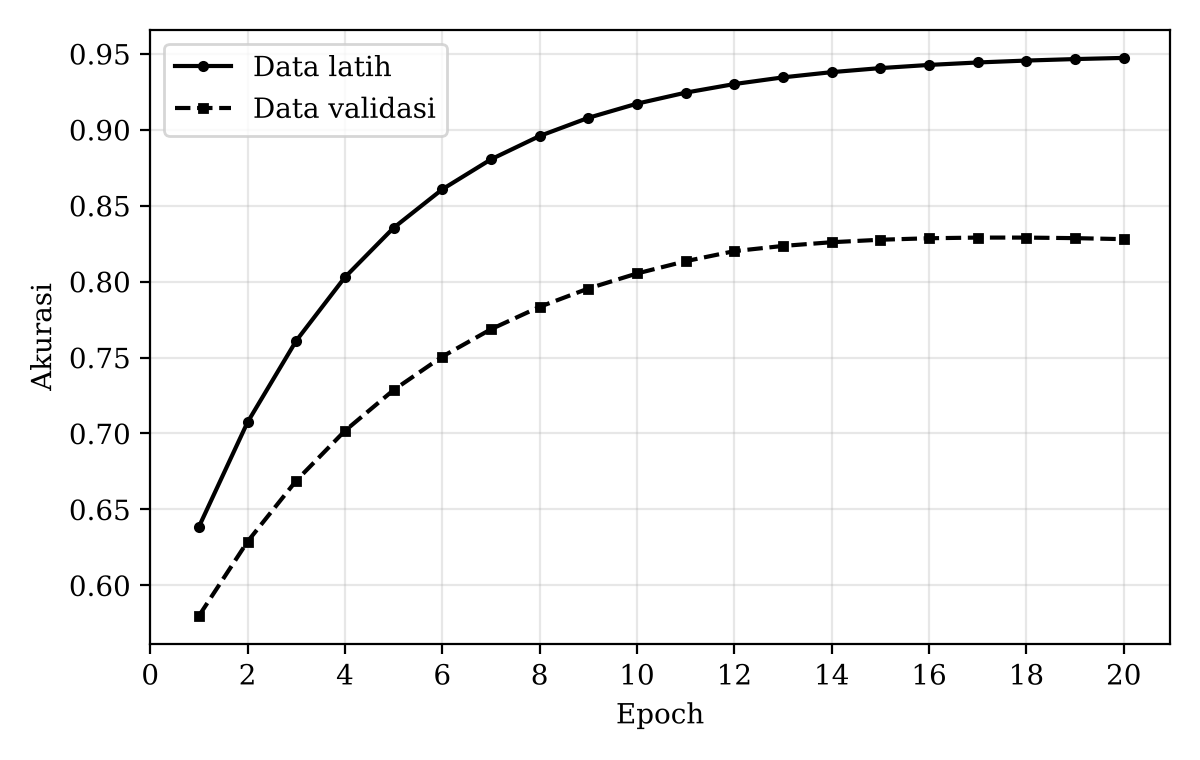
\includegraphics[width=0.8\textwidth]{grafik}
  \caption{Grafik akurasi model terhadap jumlah \asing{epoch}}
  \label{fig:grafik}
\end{figure}

\chapter{Kesimpulan dan Saran}
\section{Kesimpulan}
Uraikan kesimpulan yang menjawab rumusan masalah dan tujuan penelitian.
\section{Saran}
Uraikan saran untuk penelitian lanjutan.

%% ================================================================ daftar pustaka
\nocite{*}
\cetakdaftarpustaka

%% ================================================================ lampiran
\halamanlampiran
\lampiran{Kuesioner Penelitian}\label{lamp:kuesioner}
Isi lampiran. Setiap lampiran wajib dirujuk di dalam teks.

\lampiran{Log Prompt}
Log \asing{prompt} diletakkan sebagai lampiran terakhir bila menggunakan AI generatif kategori B atau C.

\end{document}
